I study the ways the sociotechnical architecture of a system (Figure~\ref{fig:structure}) influences remixing practices by examining these structural dimensions:
1) granularity of the remixable units, 
2) modularity of the remixable components, 
3) decomposability of a finished product, 
4) attributability mechanisms and 
5) openness to remix across systems. 
I analyze these dimensions in the large corpus of data from the Scratch Online Community and by experimenting, for example, with the system's attribution-giving mechanism.

\begin{figure}
\centering
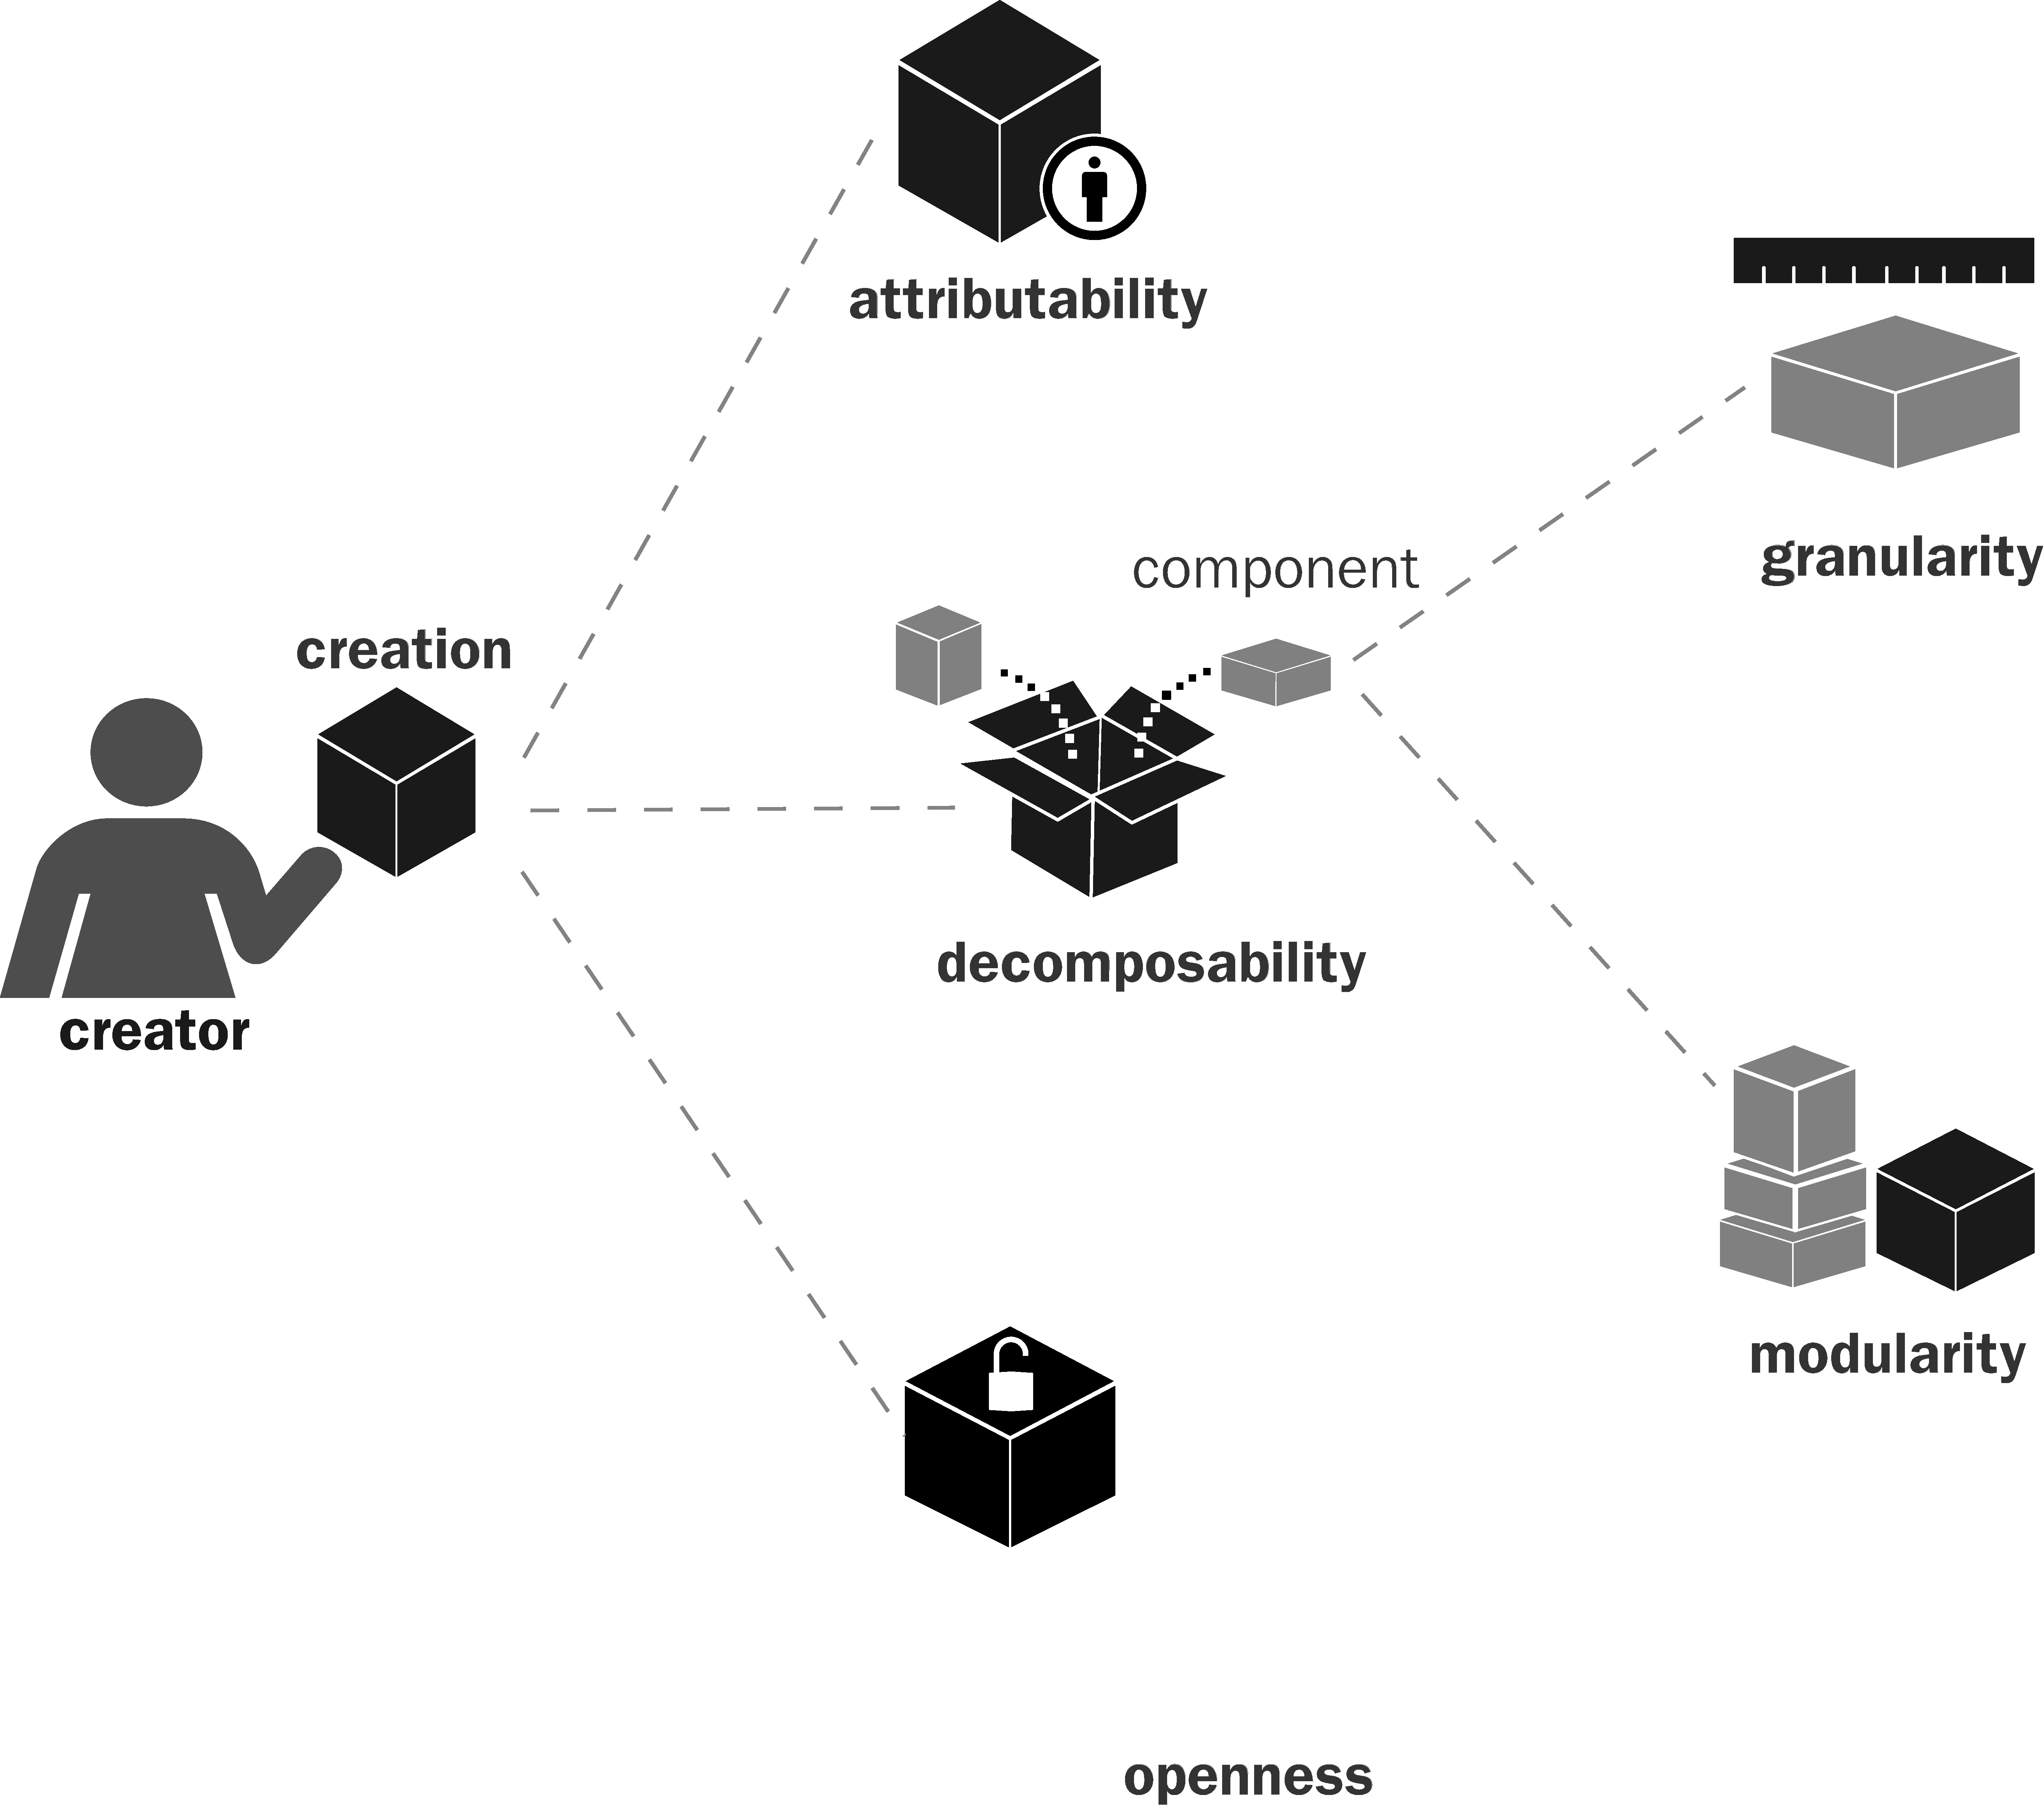
\includegraphics[width=3.25in]{figures/structure.pdf}
\caption{Structural dimensions of a remixing system}
\label{fig:structure}
\end{figure}

%  TODO: examples of each, methods for studying:
% 1. Granularity: remixing is about adding,removing,changing or mashing up. What are the size of the previous work that are reused? 
% How has that evolved over time? 
% Scratch smaller granularity is sprite but cannot be shared as such, in its place user-innovation has taken place and created ScratchResources. 
% I'll present case studies of Scratch Resources and descriptive stats on the granularity of remixed fragments and sample sprites. How memes spread and how granular they are? How granular are the components of highly remixed projects.
% Example:
% Scratch Resources
% Proposed work:
% Analyze size and adoption: adoption, spread, and size of modules of remixed projects.
% Analyze SR
% Challenges:
% - Unable to find module reuse, only project reuse

% 2. modularity: both technical and sociocultural. 
% Description:
% For example, a ball that has gravity implemented in it, can be easily repurpiosed while a complicated interconnected set of sprites and scipts in a complexly prorgammed projects are much harder to detach and modularized. 
%
% Example: 
% - Samples: sample sprites
% - Necklace: physics simulation of a string turned into a necklace. Alterative less modular version: images generated by code.
% - MHM, MakiTak: cultural modularity, reused in multiple scenarios
%
% Proposed work:
% - Look at cultural and technical modularity
% - Most modular pieces are those most remixed? Not most modular projects?
% - More modular, less learning?
% - More modular, more used?
% - Individual differences approaches to modularity: cut

% 3. decomposability.
% One of the differences between digital media and its predecesors is that it is often possible to break apart a digital creation into its components. This decomposability is not always possible however. In some cases, there are technical or legal barriers to doing so. For example, a video on YouTube is not easy to decompose into the parts that were used to making it before the editing since the source files are not uploaded while on sites like Aviary, an image can be taken apart in all its compoonents used. With software this issue has been at the forefront of the Free Software movement that advocates for complete decomposability via providing the source code along with its compiled version. 
% Using Scratch as the place to study this, we can observe that projects can be decomposed to its original parts except for its images and sounds that once.
% Rasterization, no layers, no vectors.
% Code is all decomposable to its smallest form which is the blocks.
% Analysis of decomposability of remixes. 
% Practices to prevent decomposing: obfuscation. Anti-remixing. 
% Decomposability is enforced.
% People want to share compiled code but not its components.

% 4. Attributability.
% Experiments with automatic vs credit. Responses. Results. Previous work. Future work:
% Not always desired attribution.
% - Notes 
% - Creator endorsed attribution.

% 5. Opennes.
% Across systems. Ethos explained. Creative commons version for kids. DeviatnArt conflicts
% 

